\textbf{Descripci\'on} 

El objetivo de este algoritmo desarrollado por A. Mora et al. en \cite{Mora2003} es servir de antesala a todos los dem\'as algoritmos con el fin de eliminar las implicaciones redundantes de un dataset de implicaciones antes de ser procesado por otro algoritmo. Esto conlleva una importante reducci\'on del coste computacional y temporal de la ejecuci\'on del resto de algoritmos.\\

\textbf{Reducci\'on}

Regla de la l\'ogica de Simplificaciones que nos permite reducir el tama\~no del cojunto de implicaciones.

\begin{center}
    \(\ X \to Y \vdash X \to Y \setminus X, \ donde \ Y \setminus X \neq \emptyset \)
\end{center} 

\IncMargin{1em}
\begin{algorithm}[H]
    \SetAlgoLined
    \LinesNumbered
    \DontPrintSemicolon
    \SetKw{KwOr}{or}
    \KwIn{$\Sigma$ a set of FDs; $transG$, select if transG will be applied or not}
    \KwOut{$\Sigma'$ a FDs set with less redundancy}
    \Begin{
        \ $reduction$\;
        \ $union$\;
        \Repeat{more simplifications cannot be applied} {
            \ $simp + rSimp$\;
        }
        \ Check if is possible to apply $transG$
    }%end beginre
    \caption{apply.remove.redundancy algorithm}\label{alg:1}
\end{algorithm}\DecMargin{1em}
\newpage
El proceso de eliminar implicaciones redundantes se basa en aplicar la L\'ogica de Simplificaciones \(\textbf{SL}_{FD}\) que ya hemos visto anteriormente. En este caso, lo primero a realizar es la eliminaci\'on de implicaciones cuya parte derecha est\'e vac\'ia y unir implicaciones que compartan parte izquierda (consecuente).

Lo siguiente, consiste en aplicar la simplificaci\'on y la rsimplificaci\'on de implicaciones de forma iterativa hasta que se alcance un punto fijo, es decir, cuando no se puedan simplificar m\'as implicaciones.

El \'ultimo paso consiste en aplicar la transitividad generalizada, si el usuario as\'i lo indica, lo cu\'al nos permite eliminar implicaciones que puedan ser inferidas transitivamente a partir de otras.

Para ilustrar la importancia de este algoritmo se van a ver algunos ejemplos donde se pueda apreciar el n\'umero de implicaciones que se eliminan y su importancia en la reducci\'on de coste computacional.

Destacamos que habitualmente en R se extraen implicaciones y el m\'etodo implementado en el paquete arules elimina menos redundancia en implicaciones que el algoritmo que se est\'a aqu\'i desarrollando. 

Pensamos que es un punto fuerte para el uso del paquete en muy diversas \'areas y aplicaciones. 
\newpage
\textbf{Ejemplo}

Se parte de un conjunto de 200 implicaciones (reglas de asociaci\'on con confianza 1) generadas con el algoritmo apriori a partir del dataset Mushroom incluido en el paquete arules.

\begin{figure}[H]
    \centering
    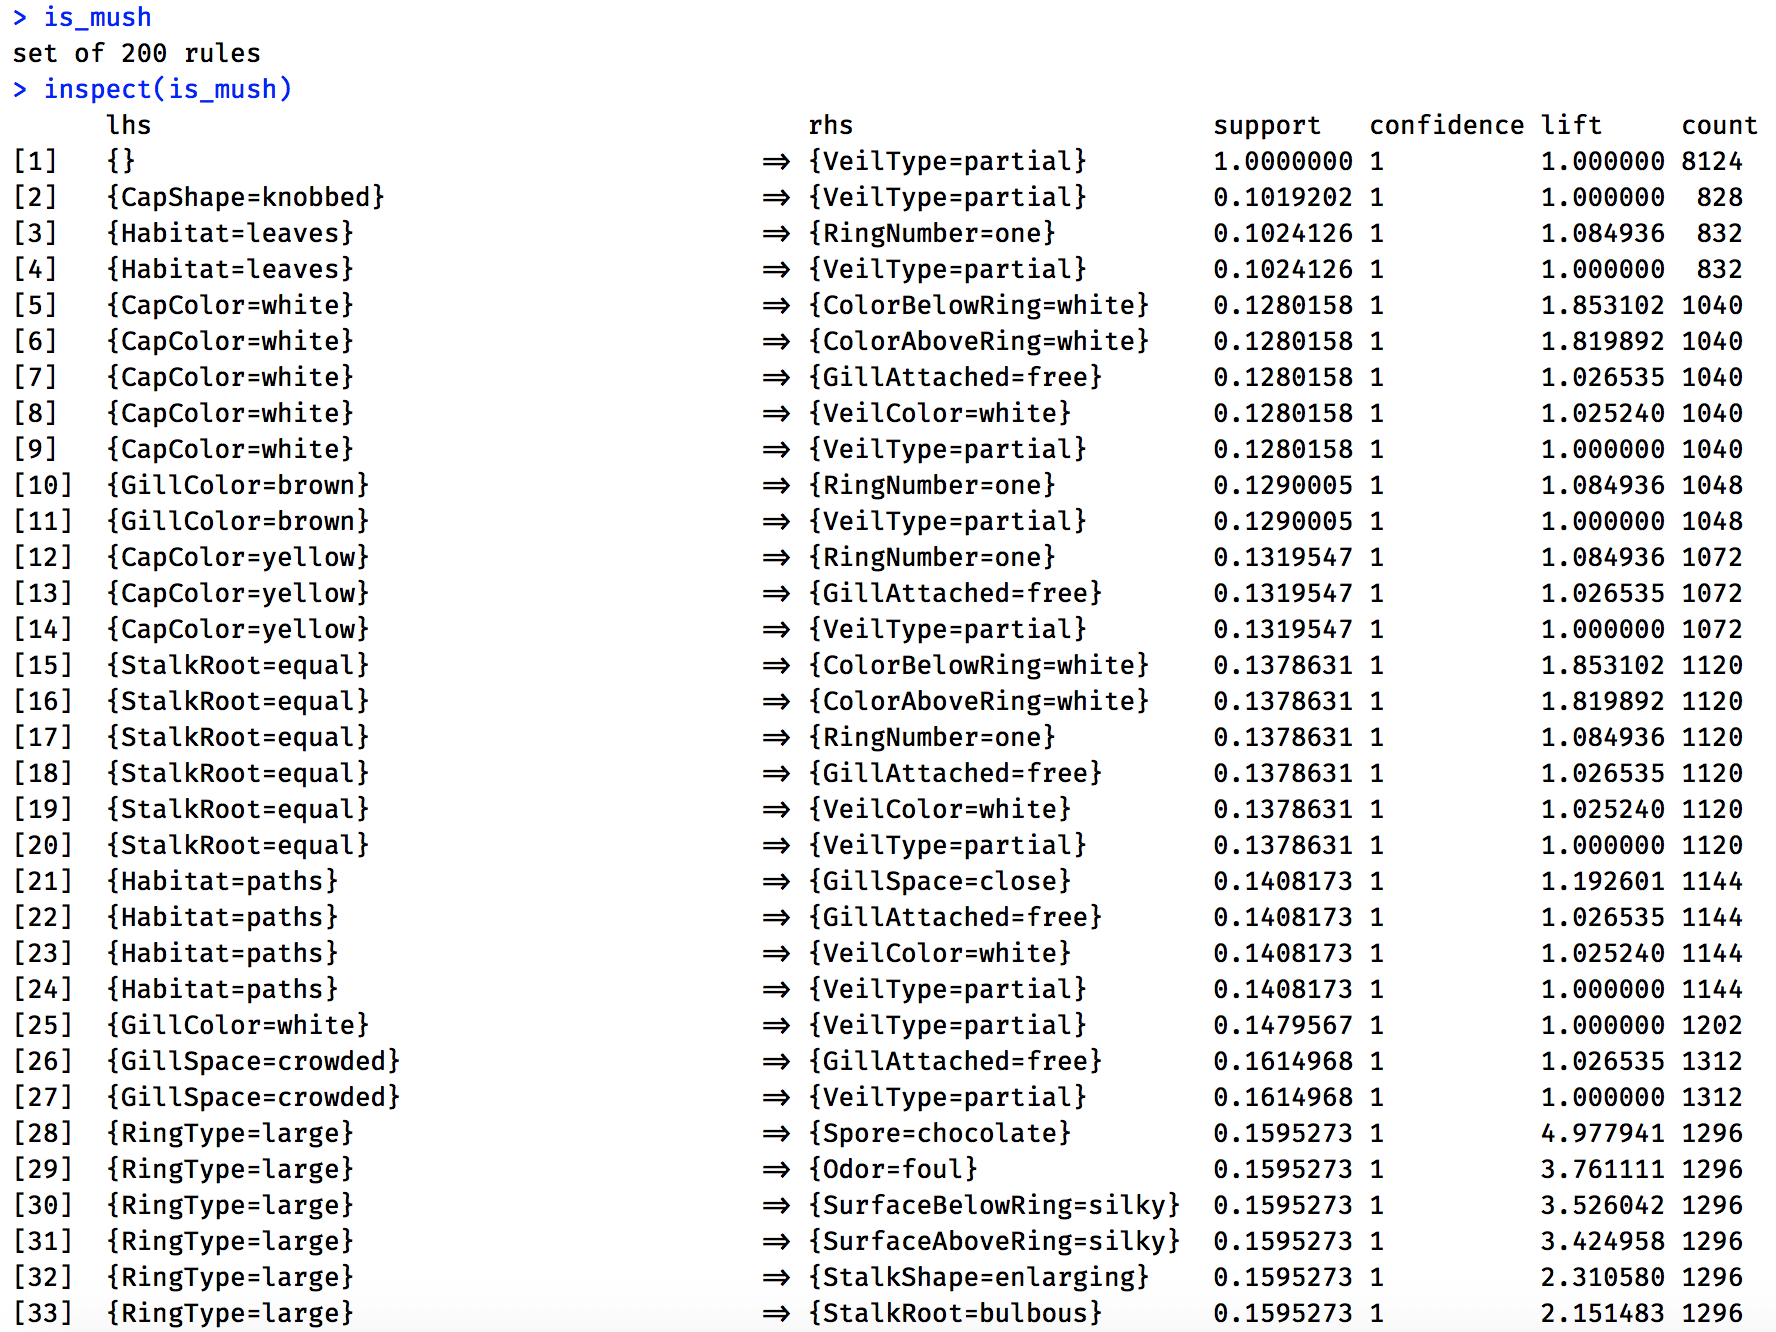
\includegraphics[scale=0.5]{red_1}
    \caption{Implicaciones Mushroom}
    \label{fig:red_1}
\end{figure} 
\newpage
A este conjunto le aplicamos el algoritmo y vemos cuantas implicaciones no redundantes se obtienen a partir del conjunto inicial.

\begin{figure}[H]
    \centering
    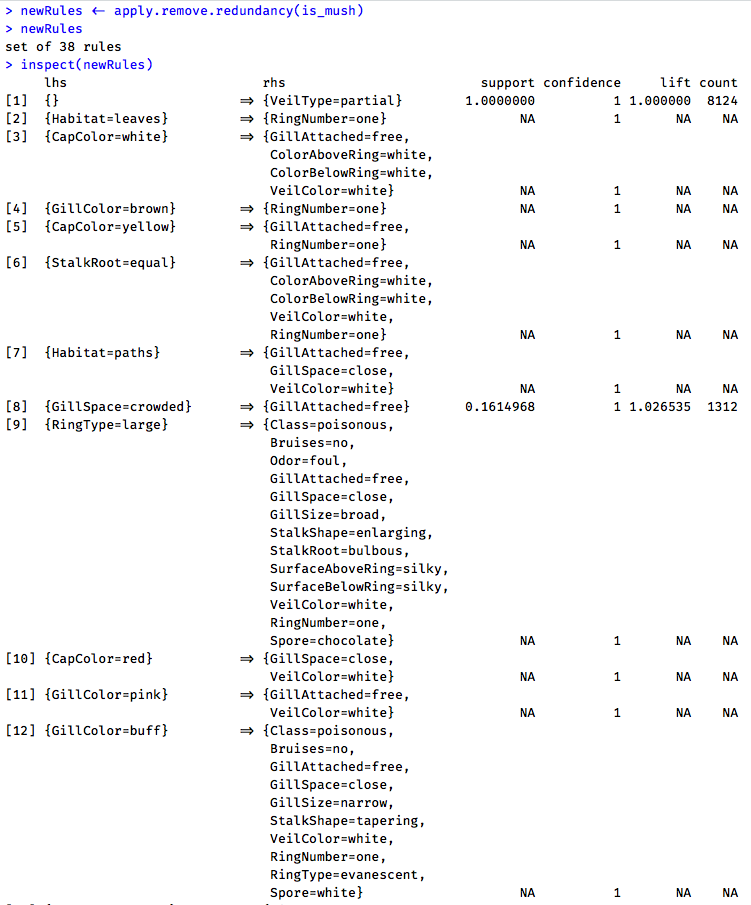
\includegraphics[scale=0.6]{red_2}
    \caption{Implicaciones Mushroom no redundantes}
    \label{fig:red_2}
\end{figure} 

Como se puede ver, de 200 implicaciones iniciales, se consigue reducir a 38 implicaciones, lo que supone una reducci\'on nada despreciable del 81 \% .

Si probamos a utilizar estos conjuntos de implicaciones con otros algoritmos, se podr\'a ver la reducci\'on del coste computacional de los otros algoritmos al trabajar con un 80\% (aproximadamente) menos de tama\~no. En este caso, se va a probar el algoritmo que calcula el cerrado de un conjunto de implicaciones a partir de un conjunto de atributos (este algoritmo se explicar\'a posteriormente).

\begin{figure}[H]
    \centering
    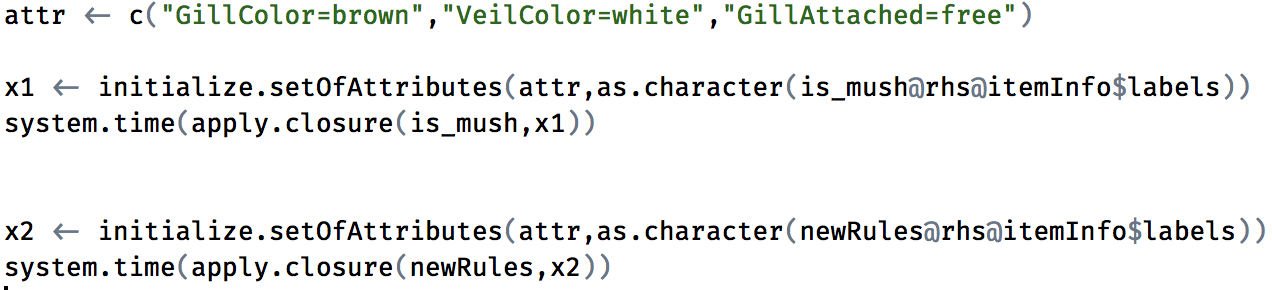
\includegraphics[scale=0.7]{red_3}
    \caption{C\'alculo del cierre}
    \label{fig:red_3}
\end{figure}

\begin{figure}[H]
    \centering
    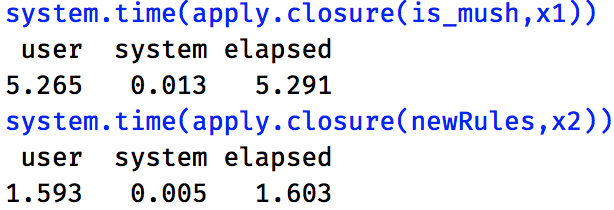
\includegraphics[scale=0.8]{red_4}
    \caption{Tiempos de c\'alculo del cierre}
    \label{fig:red_4}
\end{figure}

Aunque en este caso pueda parecer que la diferencia de tiempo es poca, se debe a que el algoritmo de c\'alculo de cierre es un algoritmo bastante r\'apido. En este caso se reduce el tiempo necesario para el c\'alculo del cierre en casi un 70 \%. Adem\'as destacamos que este dataset no contiene un n\'umero muy grande de atributos. Cuanto mayor sea el tama\~no del dataset, mayor ser\'a la mejora conseguida al aplicar cualquier algoritmo aunque sea el m\'as sencillo en t\'erminos de complejidad. 

\newpage
\textbf{C\'odigo} 
\lstinputlisting{r_code/redundancy.R}
\newpage
 
\textbf{Comparativa/Versiones} 
\begin{figure}[h]
    \centering
    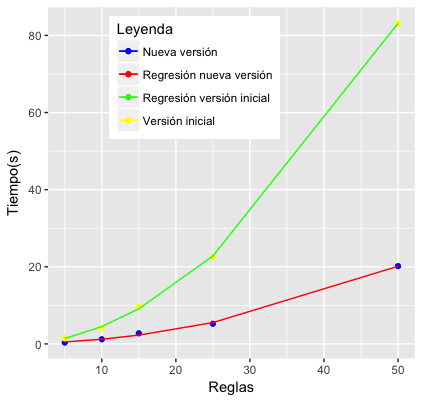
\includegraphics[scale=0.75]{Redundancy2}
    \caption{Pruebas remove.redundancy}
    \label{fig:redundancy}
\end{figure} 

En la figura \ref{fig:redundancy} se puede ver una gr\'afica comparativa entre dos versiones distintas de esta funci\'on. La primera de ellas es la versi\'on de la que dispon\'ia el director de este TFG en el momento en que se empez\'o a desarrollar el mismo. La segunda es una versi\'on mejorada (como se puede ver m\'as arriba en el extracto de c\'odigo), que se realiz\'o como parte de este trabajo. La versi\'on que exist\'ia, solo era una versi\'on pedag\'ogica del algoritmo para explicarla en congresos. El objetivo conseguido con este TFG es tener ahora una versi\'on eficiente de todos y cada uno de los algoritmos. 


Como se puede observar, la diferencia de tiempo es bastante considerable y va aumentando conforme se aumenta el n\'umero de implicaciones.